\documentclass{article}

\usepackage{microtype}
\usepackage{graphicx}
\usepackage{float}

\title{Performance and Simulation of Social Networks}
\author{Jakob Wyatt\\19477143}

\begin{document}
\maketitle
\section{Abstract}
This report presents a simple method to simulate social networks using
directed graphs, using a post propogation algorithm to model the spread
of information through this network.
These social networks exhibit behaviour that would be expected
within a real social network, despite the model being relatively simple.\\
Simulations were run to determine the most important parameters in the
success of a social network, with it being found that in the long term,
the probability of following the original poster of a post is more important
than the probability of liking the post outright.\\
An analysis of popularity and friend group clustering was also performed,
showing that friend group clusting did not change significantly over time.
It was shown that popularity of users in a network decreases over time,
however the use of clickbait within a network can change this behaviour.\\
A computationally cheap method for generating large structured graphs
is also presented within this report.\\
Finally, some potential future work and improvements relating to the simulation
algorithm are given.

\pagebreak
\section{Background}
This report focuses on simulating simple social media networks,
and evaluates the effectiveness of a network given parameters
of that network.\\
The social network consists of a set of users that may follow eachother,
which has been represented in code as a directed graph. Users may not follow themselves,
or follow eachother more than once.\\
There exists only one post at a time, with a new post being loaded when the current
post has not had any activity in the last timestep. The original poster always
likes their own post. A user can only like a post once.\\
The simulation consists
of timesteps, with a function \texttt{update()} to move between timesteps.
The update algorithm works as follows:
\begin{enumerate}
    \item Check that there exists some users that have liked the post in the previous timestep.
            If there are none, the update ends and the next post is loaded.
    \item Iterate through all users who liked the post in the previous timestep.
            Each of their followers is 'exposed' to the post, and have a chance of liking the post.
            This chance is sampled from a Bernoulli distribution with probability
            $\mathit{clamp}\left(\mathit{prob\_like} \times \mathit{clickbait\_factor}, 0, 1\right)$.
    \item If a user likes a post in the current timestep, they have a chance of following the
            original poster. This is sampled using the same technique as above, with global probability
            $\mathit{prob\_foll}$.
\end{enumerate}
Note that in the above algorithm, if a user does not like a post, they may potentially
be exposed to it later via a different friend. This behaviour is intentional, as it incentivises
a highly connected network.

Some parameters that will be varied in the creation of the social network include:
\begin{itemize}
    \item Probability of liking a post
    \item Probability of following a user
    \item Number of users
\end{itemize}

Some parameters that will be tracked throughout the simulation include:
\begin{itemize}
    \item Clustering Coefficient
    \item Average and s.d. of followers per user
    \item Likes per user per post
\end{itemize}

\section{Methodology}

Terminology in this section includes the word 'predecessor' and 'successor'
in the context of graphs. If there is a directed edge between verticies
$A \rightarrow B$, then B is a successor of A and A is a predecessor of B.

\subsection{Parameter Gridsearch}

To profile multiple runs of the simulation a gridsearch algorithm was used
to vary the below parameters:
\begin{itemize}
\item Average and s.d. of followers per user
\item Like/Follow probabilities
\item Number of users in the network
\end{itemize}

First, arrays that contain the parameter values to be tested were created.
Next, for all possible combinations of these parameters, a network
matching these parameters was created. A simulation was then run on all networks,
with simulation statistics being logged to a file in CSV format.

Parameters that are varied during the gridsearch include the like and follow probabilities,
network size, clickbait standard deviation, and
follower average / follower standard deviation.

An advantage of this algorithm is that it is very simple to implement.
However, a disadvantage is that it takes a long time to execute when there are many input parameters.
The algorithmic complexity of the gridsearch algorithm
is $O(x^n)$, where n is the number of parameters that are varied and x is the number
of datapoints per parameter.

\subsection{Statistics}
Throughout the simulation, various statistics about the state of the network were
computed. These included the average/s.d. followers per user and the average number of likes
per user.
One particularly interesting statistic that was calculated was the Clustering Coefficient.
To calculate the clustering coefficient of a vertex $V$, the neighbourhood of that
vertex is first found.\\
$N = V_{successors} \bigcup V_{predecessors}$\\
Next, the number of connections between nodes in this neighbourhood is found.\\
$C = |{e_{jk} : v_j, v_j \in N, e_{jk} \in E}|$\\
Finally, this is divided by the total number of potential connections within the neighbourhood.\\
$\mathit{Clustering Coefficient} = \frac{C}{|N| \times (|N| - 1)}$\\
To find the network average clustering coefficient, the clustering coefficient
is calculated for all verticies in the network and averaged.
As the number of followers will always increase over time in this simulation,
to enable comparison between clustering coefficients at different timesteps,
the network average clustering coefficient was then divided by the number
of edges in the graph.
This algorithm has $O\left(n^3\right)$ execution time when hashtables are used to store
edges and verticies, which is done in this program.
When a linked list is used instead, this execution time degrades to $O\left(n^4\right)$.

\subsection{Graph Generation}

To generate the simulated networks, a unique algorithm was used
that was created by the author, and to their knowledge, does not exist anywhere else.
This algorithm allows efficient generation of structured (non-random) networks,
with a consistent runtime complexity of $O\left(V \times E\right)$.

First, a number of verticies are created.
Next, these verticies are iterated over, and the number of successors of each
vertex is calculated by sampling from a distribution $X \sim N\left(follower\_av, follwer\_sd^2\right)$.

To select the edges of the network, an approach was used that is similar in concept
to a variogram, used in the field of geostatistics.
A variogram measures the amount of correlation between two points in a field that are some distance apart.
In this algorithm, this distance is discrete rather than continuous, and is measured by finding
a path between two nodes. By increasing the correlation between nodes at short distances,
a graph can be created with a higher clustering coefficient. Alternatively,
decreasing the correlation between nodes causes the graph to become more randomised,
and less clustered.

The clustering coefficient of a vertex can be generalized to include all verticies
within some distance $h$ of a central vertex (Xiao et al. 2007), rather than
only verticies within a distance of 1 of the central vertex.

In a social network, it is reasonable to assume that the clustering
coefficient will decrease as the distance increases.
One way to visualise this is that your friends are likely to be interconnected,
whereas your friends of friends are less likely to be interconnected directly.
By creating graphs that follow this property, realistic social networks
can be created for use in simulations.

To generate an edge in the graph, a random walk is performed starting at a given vertex, $V_0$.
This random walk occurs along any nodes that are predecessors of the current node,
and does not loop back onto previously visited nodes.
At each step on the random walk, the probability of creating an edge between the current node and $V_0$
is calculated by evaluating the variogram $\gamma (h)$, where h is the distance that has been travelled on the random walk.

If an edge is created, a new random walk begins starting at the vertex $V_0$,
and this algorithm repeats until the correct number of edges have been created
for this vertex.
If there are no valid verticies to walk to,
or the random walk has reached some distance threshold from the original node,
an edge is created with any random vertex in the graph. This allows initial
'bootstrapping' of the network when no edges have yet been created.

\subsection{Time and Space Complexity}
The core algorithm that propogates a post through the network has a time complexity of
$O\left(V \times E\right)$ per timestep.
However, many algorithms that calculate network statistics have a much
worse time complexity. One example is the calculation of the clustering coefficient,
which has a time complexity of $O\left(V^3\right)$ when implemented using a hash table.
The space complexity of this program is $O\left(V + E\right)$. Although
a large amount of caching is used to speed up the program, none of this caching
is non-linear in the size of the input data.

\subsection{Execution}
The generated data for this simulation can be found in report/subset.csv.
This data can be created by executing the below command, found in the \texttt{src} directory:\\
\texttt{python3 SocialNetworkSimRunner.py}\\
This program takes approximately 14 minutes to run on an i7-7700k processor,
and requires 170 MB of memory.

To modify the parameters of the gridsearch algorithm,
simply edit the array variables at the beginning of the \texttt{Gridsearch}
function, found in the file \texttt{SocialNetworkSimRunner.py}.

\section{Results}

It was found that clustering coefficient did not change significantly over the
course of the simulation, and either increases or decreases by a maximum of 10\%.
This shows that over time, friend groups within the network do not increase
or decrease the amount of connections within the group, relative to all other connections.

Average followers per person, as well as likes per person, all increased over time.
This was expected, as there is no mechanism for unliking a post or unfollowing a user
during a simulation. These statistics appeared to increase exponentially;
however, this behaviour could only be observed when the like and follow probabilities
were low, and the graph was relatively large. With a high probability, such as 0.5, posts often 'saturate' the network,
and give data that is not representative of a real life situation.
\begin{figure}[H]
\centering
\begin{minipage}{.5\textwidth}
  \centering
  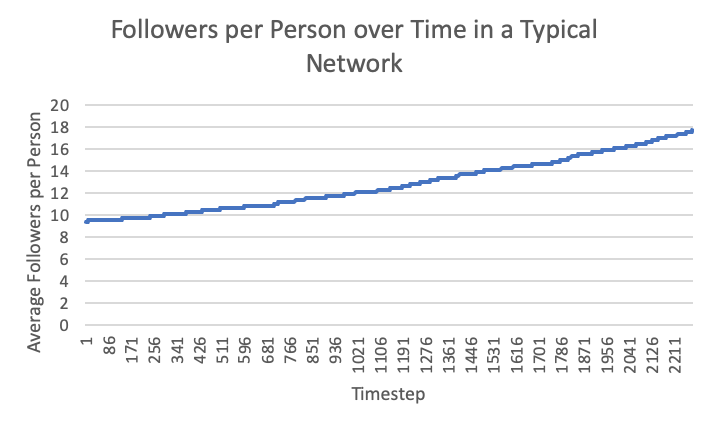
\includegraphics[width=\linewidth]{follAv}
\end{minipage}\hfill
\begin{minipage}{.5\textwidth}
  \centering
  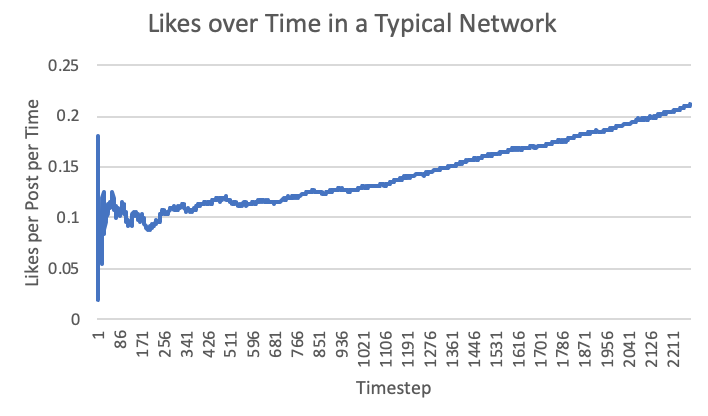
\includegraphics[width=\linewidth]{likes}
\end{minipage}
\end{figure}

Follower standard deviation also increased over time. However, when scaled with respect
to the total number of followers, it was observed to decrease over time,
eventually reaching a stable value after a long time.
An exception of this rule is networks with initial follower s.d. = 0,
where the follower s.d. quickly rises to a low, stable value.
Follower s.d. is analagous to the amount of 'inequality', or 'fame',
within a network, as a high s.d. means there is greater variation in the number
of followers across the network.
This result shows that fame within a network generally decreases over time,
and is a result of the network eventually reaching a state of equilibrium.

When the standard deviation of the clickbait factor was increased, the follower s.d. reached
a higher stable value than when the network was simulated without clickbait.
However, when this was done with an initially random graph, the follower s.d.
did not end up being as high.
This shows that use of clickbait is an effective
tool to retain fame within a network, however cannot be used to
create fame within a network.

\begin{figure}[H]
\centering
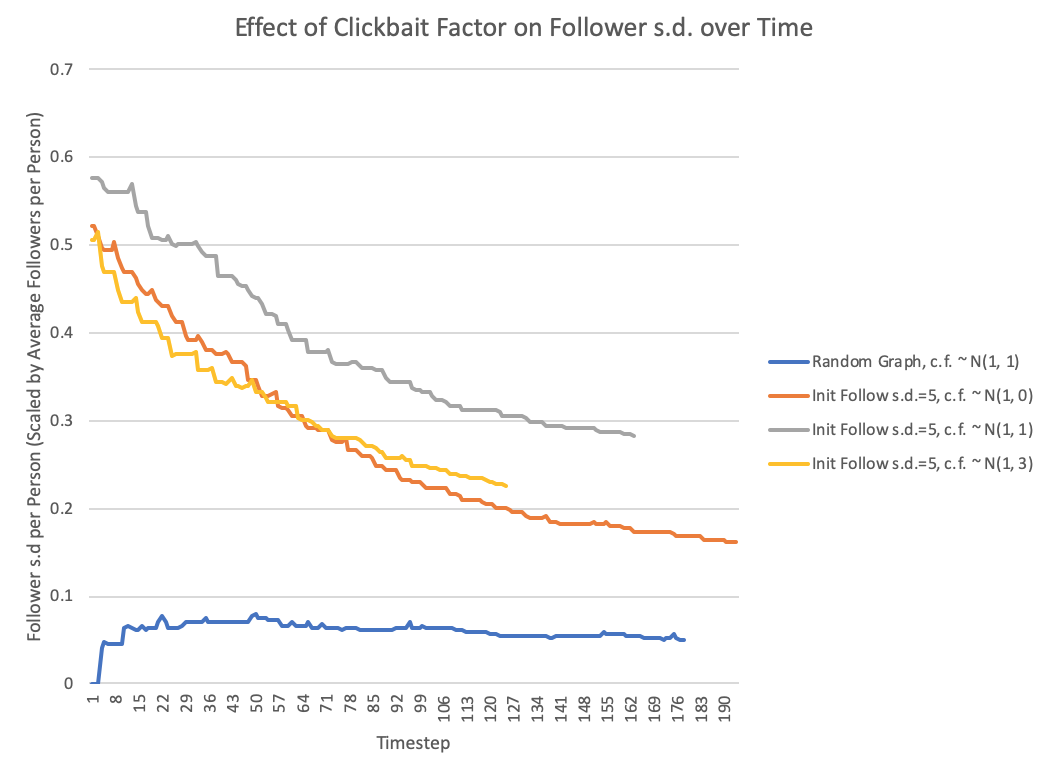
\includegraphics[width=.7\linewidth]{follSd}
\end{figure}

Another question that can be asked about a social network is
the tradeoff between the like probability and the follow probability.
If the follow probability is low, the user base will stagnate and there will
not be as much growth within the network.
In contrast, if the like probability is low, users will not like posts
and they will not propogate through the network as effectively.
What is the best tradeoff between these two options?

\begin{figure}[H]
\centering
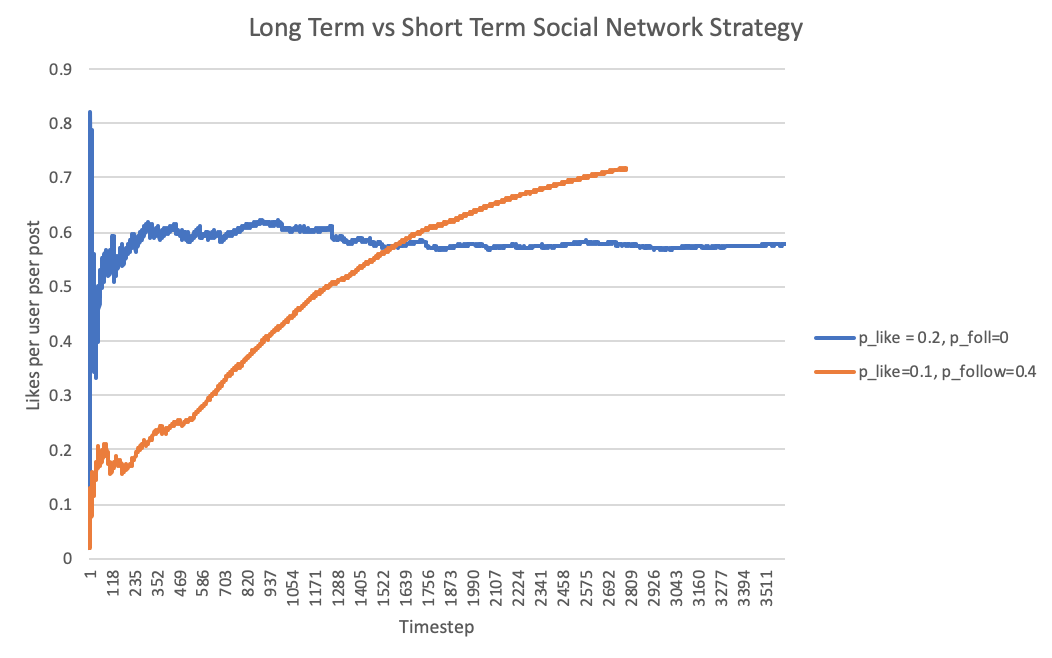
\includegraphics[width=.7\linewidth]{Growth}
\end{figure}

It can be seen from the above graphs that despite having a higher like probability,
the blue network eventually stagnates and does not grow. Because of this,
it is eventually beat by the orange network, which started out with a lower like probability,
but had a higher follow probability.

This shows that when creating a social network, showing content that is relevant
to the user may help to grow the platform long term. Although showing 
popular non-personalized content to the user will increase the short term probability of liking a post,
they may be less likely to follow the original poster.
In contrast to this, showing less popular but more personalized content to a user
may increase the probability that they follow the original poster, which leads
to long term growth in a social network.

\section{Conclusion and Future Work}
Despite being simple, the social network model and algorithm that was used
in this assignment was still able to exhibit many of the properties
that would be expected in a real social network.
By using this model to run simulations of a social network, the affect of
clickbait, fame, and friend groups on a social network were analysed.\\

One application of the code written in this report could be to predict the outcome
of changes to a social media network before these changes are implemented.
This could be used to help analyse strategies within a social media company.
Another potential application of this simulation could be to model the spread of disease
within a population.\\

Future work that could be done to improve this simulation and analysis involve both better
analysis of the current data, generation of testing networks using different algorithms,
and implementing more graph statistics to measure.\\

Due to time constraints, only a limited amount of basic analysis could be done
on generated data. This analysis was mostly constrained to setting constant values for certain
parameters, and varying a single parameter at a time to see the outcome.
This assumes that each parameter is independent, however this may not be the case.

A more in-depth analysis could involve principal component analysis to rigorously
determine the most important factors in the performance of a social network.\\

The current algorithm used to generate random graphs with structure is not mathematically rigorous.
One method of verifying the results of this algorithm would be to implement a different
graph generation algorithm, such as ClustRNet (Bansal, Khandelwal, and Meyers, 2009),
and compare the results of the two methods. This was not done
as it is outside the scope of this report.\\

Only a small amount of statistics related to graphs were analysed. To improve this
analysis in future, a wider range of statistics about the graph could be calculated at each time step,
including but not limited to:
\begin{itemize}
\item Mutuality (The probability that a user is followed back)
\item Distance (The minimum number of edges required to connect any two verticies in the graph)
\item Centrality of highly followed users (How much influence does a node have)
\end{itemize}
This would allow a more in depth analysis into the factors behind social network performance, and a better
comparison with real life networks.\\

One way to potentially increase the applicability of this simulation code could
be to increase the complexity of the model. One example of this could be to 
have a different like probability for each user in the network.
However, this added complexity would not be worth the implementation time required,
with the previous three suggestions offering greater benefit for less development
time.

\section{References}
Xiao, Wenjun, Wenhong Wei, Weidong Chen, Yong Qin, Behrooz Parhami. 2007.
\textit{Extended Clustering Coefficients: Generalization of Clustering Coefficients in Small-World
Networks}. Journal of Systems Science and Systems Engineering. https://www.ece.ucsb.edu/~parhami/pubs\_folder/parh07-jssse-ext-clustering-coeff.pdf\\

Bansal, Shweta, Shashank Khandelwal, and Lauren Ancel Meyers. 2009. \textit{Exploring Biological Network Structure with Clustered Random Networks}.
BMC Bioinformatics. https://bmcbioinformatics.biomedcentral.com/articles/10.1186/1471-2105-10-405



\end{document}
